\\ \lesson{21}{24/04/2020}Now let's consider a (arithmetic, not geometric) Brownian motion with a linear drift $\mu$:
\begin{equation}\label{211}
    \begin{cases}
    \dd X(t) = \mu\dd t + \sigma\dd W(t) \\
    X(0) = \alpha
    \end{cases}
\end{equation}
with $\mu,\sigma$ constants. We want to compute the hitting time: the idea is to change the probability measure in such a way that the drift is absorbed in a shift of the BM. \\
Solving \eqref{211} we get:
\begin{equation}
    X(t) = \alpha + \mu t + \sigma W(t) = \alpha + \sigma\left(\theta t + W(t)\right)
\end{equation}
where $\theta = \nicefrac{\mu}{\sigma}$. Now we change the BM
\begin{equation}\label{ww}
    W(t)+\theta t \equiv \Tilde{W}(t)
\end{equation}
in such a way that under the new probability measure $\Tilde{\Pmeas}$ associated to $\Tilde{W}$ there is no drift:
\begin{equation}\label{212}
    X(t) = \alpha + \sigma\Tilde{W}(t)
\end{equation}
The corresponding Radon-Nikodym derivative is:
\begin{equation} % remark in the notes
    \eval{\frac{\dd\Tilde{\Pmeas}}{\dd\Pmeas}}_t = \exp{-\theta W(t) - \frac{1}{2}\theta^2 t}
\end{equation}
Let's define the hitting time for the BM with drift as:
\begin{equation}
    T_{\beta} = \inf\{t:X(t)=\beta\} \overset{\eqref{212}}{=} \inf\bigg\{t: \Tilde{W}(t) = \frac{\beta-\alpha}{\sigma}\bigg\}
\end{equation}
Now we can compute the probability:
\begin{align}\label{213}
    \Pmeas\left(\max_{s\le t}X_s \ge \beta\right) = \mathbb{E}^{\Pmeas}[\mathds{1}_{T_{\beta}\le t}]
\end{align}
Recall that the expected value of a given process $Y$ is given by:
\begin{equation*}
    \mathbb{E}^{\Pmeas}[Y] = \int Y \dfrac{\dd\Pmeas}{\dd\Tilde{\Pmeas}}\dd\Tilde{\Pmeas} = \mathbb{E}^{\Tilde{\Pmeas}}\left[\frac{\Pmeas}{\Tilde{\Pmeas}}\right]
\end{equation*}
so we have to consider the converse of the Radon-Nikodym derivative:
\begin{align}
    \notag\eqref{213} &= \mathbb{E}^{\Tilde{\Pmeas}}\left[e^{\theta W(t) + \frac{1}{2}\theta^2 t}\mathds{1}_{T_{\beta}\le t}\right] \\
    \overset{\eqref{ww}}&{=}
    \notag\mathbb{E}^{\Tilde{\Pmeas}}\left[e^{\theta \Tilde{W}(t) - \frac{1}{2}\theta^2 t}\mathds{1}_{T_{\beta}\le t}\right] \\
    &=
    \notag\mathbb{E}^{\Tilde{\Pmeas}}\left[\mathbb{E}^{\Tilde{\Pmeas}}\left[e^{\theta \Tilde{W}(t) - \frac{1}{2}\theta^2 t}\mathds{1}_{T_{\beta}\le t}\right]\bigg\vert\mathcal{F}_{t\wedge T_{\beta}}\right] \\
    &=
    \notag\mathbb{E}^{\Tilde{\Pmeas}}\left[e^{\theta\frac{\beta-\alpha}{\sigma} - \frac{1}{2}\theta^2 t}\,\mathds{1}_{T_{\beta}\le t}\right] \\
    &=
    \notag\int_0^t e^{\theta\frac{\beta-\alpha}{\sigma} - \frac{1}{2}\theta^2 y}\, \Tilde{\Pmeas}(T_{\beta}\in\dd y) \\
    \overset{\eqref{hittimedens}}&{=}
    \notag\int_0^t e^{\theta\frac{\beta-\alpha}{\sigma} - \frac{1}{2}\theta^2 y}\frac{\frac{\beta-\alpha}{\sigma}}{\sqrt{2\pi y^3}}e^{-\frac{1}{2y}\left(\frac{\beta-\alpha}{\sigma}\right)}\,\dd y \\
    &=
    \int_0^t \frac{\beta-\alpha}{\sigma}\dfrac{1}{\sqrt{2\pi y^3}}\exp{-\frac{\left(\tfrac{\beta-\alpha}{\sigma}-\theta y\right)^2}{2y}}\,\dd y
\end{align}
Summarizing, we found that for a BM $X(t) = \alpha + \mu t + \sigma W(t)$ with drift the probability of its maximum to be greater of equal to $\beta$, such that $T_{\beta}=\inf\{t:X(t)=\beta\}$, is given by:
\begin{equation}
    \Pmeas\left(\max_{s\le t}X_s \ge \beta\right) = \int_0^t \frac{\beta-\alpha}{\sigma}\dfrac{1}{\sqrt{2\pi y^3}}\exp{-\frac{\left(\tfrac{\beta-\alpha}{\sigma}-\theta y\right)^2}{2y}}\,\dd y
\end{equation}
where $\theta = \nicefrac{\mu}{\sigma}$.
\begin{example}{}{}{} % typical intership question 1
    Consider the exponential martingale
    \begin{equation}
        Y(t)=e^{W(t)-\frac{1}{2}t}
    \end{equation}
    and the stopping time
    \begin{equation}
        \tau_n = \inf\{t:Y(t) = n\}, \qquad n\in\mathbb{N}
    \end{equation}
    We would like to understand which is the probability
    \begin{equation}
        \Pmeas(Y(t)=n \text{ for some } t) =\, ?
    \end{equation}
    The problem is that $Y(t)$ is not uniformly integrable (UI)\footnote{The criterion for the uniform integrability is that $\lim_{M\to\infty}\sup_{t}\mathbb{E}[X(t)\mathds{1}_{\abs{X(t)}>M}]=0$. This condition is quite difficult to verify. The usual predure consists in bounding the martingale. If the martingale is bounded, then it is UI.}. In fact,
    \begin{equation*}
        \lim_{t\to\infty}Y(t) = \lim_{t\to\infty}e^{t\left(\frac{W(t)}{t}-\frac{1}{2}\right)} = 0
    \end{equation*}
    and so
    \begin{equation*}
        1 = \mathbb{E}[Y(t)] \ne \mathbb{E}[Y(\infty)] = 0
    \end{equation*}
    So, since there is no convergence, the martingale is not uniform integrable. The idea to solve this problem is to exploit the UI of a particular version of this exponential martingale. Let's consider the exponential martingale computed at time $t\wedge\tau_n$: $Y(t\wedge\tau_n)$. Being a martingale stopped at a bounded time, this is still a martingale. If we consider the limit, we get:
    \begin{equation}\label{lim11}
        \lim_{t\to\infty} Y(t\wedge\tau_n) =
        \begin{cases}
        0 & \text{if } \nexists t : Y(t) = n \\
        n & \text{if } \exists t : Y(t) = n
        \end{cases}
    \end{equation}
    We found that the martingale $Y(t\wedge \tau_n)$ is bounded both from above (by $n$) and below (by construction) and so it is UI and it converges:
    \begin{equation*}
        1 = \mathbb{E}[Y(t)] = \mathbb{E}[Y(\infty\wedge\tau_n)] \overset{\eqref{lim11}}{=} n\Pmeas(Y(t)=n \text{ for some } t) + 0
    \end{equation*}
    Solving this equation we get:
    \begin{equation}
        \Pmeas(Y(t)=n \text{ for some } t) = \frac{1}{n}.
    \end{equation}
\end{example}
\begin{example}{}{}{} % typical intership question 2
    Consider two real numbers $a,b>0$, a BM $B(t)$ and the first hitting time
    \begin{equation}
        T = \inf\{t:B(t) = -a \text{ or } B(t) = b\} = T_{-a}\wedge T_{b}
    \end{equation}
    \begin{center}
        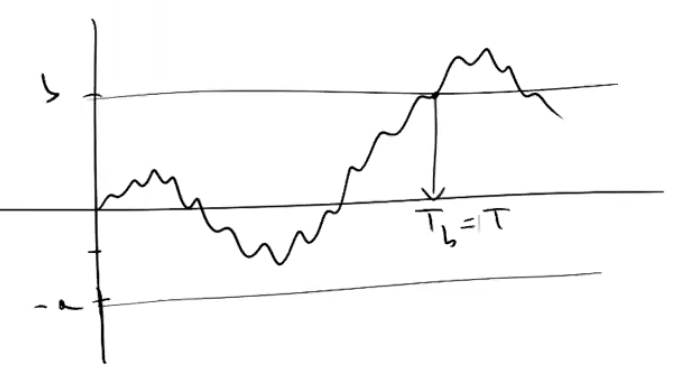
\includegraphics[scale=0.26]{fig/tmp/fig35.png}
    \end{center}
    We want to compute $\mathbb{E}[T]$. Since $T$ is bounded, we have to construct something which is bounded. We know that, by construction, $\abs{B(t)}\le\max\{a,b\}$. Then, from the optional stopping theorem, $B_{t\wedge T}$ is a martingale, so it is UI. By martingality we have that the expected value of $B_{t\wedge T}$ is equal to the initial value, which is zero:
    \begin{equation*}
        0 = \mathbb{E}[B_{t\wedge T}]
    \end{equation*}
    So, if we consider the limit, we have:
    \begin{align}\label{lim22}
        \notag 0 &= \lim_{t\to\infty}\mathbb{E}[B_{t\wedge T}] = \mathbb{E}\left[\lim_{t\to\infty} B_{t\wedge T}\right] = \mathbb{E}[B(T)] \\
        &=
        \notag -a\Pmeas(B(T)=-a) + b\Pmeas(B(T)=b) + (?)\Pmeas(B(\infty)\in(a,b)) \\
        &=
        -a\Pmeas(B(T)=-a) + b\Pmeas(B(T)=b)
    \end{align}
    where the last term stands for the case in which the BM will always remain inside the interval $(a,b)$ and it is zero because the BM has infinite upper and lower limit. From \eqref{lim22} we conclude that the two events are exclusive:
    \begin{equation}
        \Pmeas(B(T)=b) = 1 - \Pmeas(B(T)=-a)
    \end{equation}
    Moreover, we can rewrite \eqref{lim22} as:
    \begin{equation}
        0 = -a(1-\Pmeas(B(T)=b) + b\Pmeas(B(T)=b)
    \end{equation}
    so that
    \begin{equation}\label{214}
        \Pmeas(B(T)=b) = \frac{a}{b}\frac{1}{1-\frac{a}{b}} = \frac{a}{a+b} \quad\Rightarrow\quad \Pmeas(B(T)=-a) = \frac{b}{a+b}
    \end{equation}
    $\Pmeas(B(T)=b)$ is called \emph{gain probability} and $\Pmeas(B(T)=-a)$ \emph{ruin probability}. \\
    Now we use another martingale, which is $B(t)^2 - t$. By the optional stopping theorem we have that
    \begin{equation}
        B(t\wedge T)^2 - (t\wedge T) = \text{martingale}
    \end{equation}
    and by martingality we get:
    \begin{equation}
        \mathbb{E}[B(t\wedge T)^2] = \mathbb{E}[t\wedge T]
    \end{equation}
    Now, recalling that $B(t\wedge T)^2 \le \max\{a^2,b^2\}$, if we take the limit for $t$ going to infinite we get:
    \begin{equation}\label{215}
        \mathbb{E}[B(T)^2] = \mathbb{E}[T]
    \end{equation}
    So we are able to express the expected value we want to compute in terms of a discrete random variable which takes values $a^2,b^2$. Using eq. \eqref{214} we can write eq. \eqref{215} as:
    \begin{equation}
        a^2\frac{b}{a+b} + b^2\frac{a}{a+b} = \mathbb{E}[T]
    \end{equation}
    Thus, we get:
    \begin{equation}
        \mathbb{E}[T] = ab.
    \end{equation}
\end{example}

\subsection{Barrier options: a classic approach}
Consider a B\&S model in which the underlying under the risk neutral probability measure is given by
\begin{align}
    \notag S(t) &= S(0)\exp{\left(r-\frac{1}{2}\sigma^2\right)t + \sigma B^{\Qmeas}(t)} \\
    &=
    \notag S(0)\exp{\sigma\left(\left(\frac{r}{\sigma}-\frac{\sigma}{2}\right)t + \sigma B^{\Qmeas}(t)\right)} \\
    \overset{(a)}&{=}
    S(0)\exp{\sigma\Tilde{B}^{\Qmeas}(t)}
\end{align}
where in (a) we defined
\begin{equation}
    \theta \equiv \frac{r}{\sigma}-\frac{\sigma}{2} \quad \text{ and } \quad \Tilde{B}^{\Qmeas}(t) \equiv B^{\Qmeas}(t) + \theta t
\end{equation}
Let's define the running maximum as
\begin{equation}
    M^S(t) = \max_{s\le t} S_s = S(0)\exp{\sigma M^{\Tilde{B}}(t)}
\end{equation}
In order to price something which involves the past trajectory of the underlying, we need to consider the joint probability of the running maximum and the current value of the underlying:
\begin{align}
    \notag\Qmeas(M^S(t)\le L,S(t)\ge K) &= \expect[\mathds{1}_{M^S(t)\le L,S(t)\ge K}] \\
    &=
    \expect\left[\mathds{1}_{M^{\Tilde{B}}(t)\le\frac{1}{\sigma}\ln{\frac{L}{S(0)}}, \Tilde{B}(t)\ge\frac{1}{\sigma}\ln{\frac{K}{S(0)}}}\right]
\end{align}
Now we move from the probability measure $\Qmeas$ to $\Tilde{\Qmeas}$, under which $\Tilde{B}(t)$ is a BM. The corresponding Radon-Nikodym derivative is:
\begin{equation}
    \eval{\frac{\dd\Tilde{\Qmeas}}{\dd\Qmeas}}_t = e^{-\theta B(t)-\frac{1}{2}\theta^2 t} \qquad\Rightarrow\qquad \eval{\frac{\dd\Qmeas}{\dd\Tilde{\Qmeas}}}_t = e^{\theta B(t)+\frac{1}{2}\theta^2 t} = e^{\theta\Tilde{B(t)}-\frac{1}{2}\theta^2 t}
\end{equation}
This change of measure leads to:
\begin{equation}
    \Qmeas(M^S(t)\le L,S(t)\ge K) = \mathbb{E}^{\tilde{\Qmeas}}\left[e^{\theta\Tilde{B(t)}-\frac{1}{2}\theta^2 t} \mathds{1}_{M^{\Tilde{B}}(t)\le\frac{1}{\sigma}\ln{\frac{L}{S(0)}}, \Tilde{B}(t)\ge\frac{1}{\sigma}\ln{\frac{K}{S(0)}}}\right]
\end{equation}
Let's apply this result to an example.

\subsubsection{Up-and-out call}
The \emph{Up-and-out call} (UOC) is a type of knock-out\footnote{A knock-out option is an option with a built-in mechanism to expire worthless if a specified price level in the underlying asset is reached.} barrier option that ceases to exist when the price of the underlying rises above a specific price level, called barrier price. In other words, we get the payoff of the call only if the underlying never reaches a certain upper level $L$:
\begin{equation}
    \pay_T(\uoc) = (S(T)-K)^+\mathds{1}_{S(T)<L\,\forall t\le T}
\end{equation}
There are two possible situations:
\begin{enumerate}
    \item $K<S(0)<L$;
    \item $S(0)<K<L$.
\end{enumerate}
In fact, the case $K>L$ is financially meaningless, because the payoff is zero. \\
Let's consider the case in which $S(0)<K<L$.
\begin{figure}[h]
    \centering
    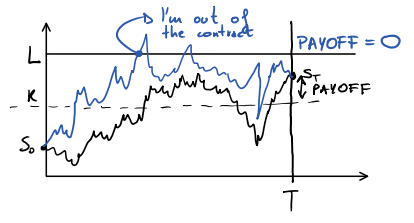
\includegraphics[scale=0.35]{fig/tmp/fig36.png}
    \caption{Case in which $S(0)<K<L$.}
    \label{fig:uoc}
\end{figure}
The price of the UOC is given by:
\begin{align}
    \notag price_0(\uoc) &= e^{-rt}\expect[(S(T)-K)^+\mathds{1}_{M^S(T)<L}] \\
    &=
    \notag e^{-rt}\expect[(S(0)e^{-\sigma \Tilde{B}(t)}-K)\mathds{1}_{M^{\Tilde{B}}(t)\le\frac{1}{\sigma}\ln{\frac{L}{S(0)}}, \Tilde{B}(t)\ge\frac{1}{\sigma}\ln{\frac{K}{S(0)}}}] \\
    &=
    \notag e^{-rt}\mathbb{E}^{\Tilde{\Qmeas}}[e^{\theta\Tilde{B(t)}-\frac{1}{2}\theta^2 t} (S(0)e^{-\sigma  \Tilde{B}(t)}-K)\mathds{1}_{M^{\Tilde{B}}(t)\le\frac{1}{\sigma}\ln{\frac{L}{S(0)}}, \Tilde{B}(t)\ge\frac{1}{\sigma}\ln{\frac{K}{S(0)}}}] \\
    \overset{(a)}&{=}
    \notag e^{-rt}\int_{\frac{1}{\sigma}\ln{\frac{K}{S(0)}}}^{\frac{1}{\sigma}\ln{\frac{L}{S(0)}}}\dd b \int_b^{\frac{1}{\sigma}\ln{\frac{L}{S(0)}}} e^{\theta b-\frac{1}{2}\theta^2 T} (S(0)e^{-\sigma b}-K)(\text{JD})\,\dd m \\
    \overset{(b)}&{=}
    \notag e^{-rt}\int^{\Tilde{m}}_{\Tilde{b}}\dd b \int^{\Tilde{m}}_{b}e^{\theta b-\frac{1}{2}\theta^2 T} (S(0)e^{-\sigma b}-K) \frac{2(2m-b)}{\sqrt{2\pi t^3}}e^{-\frac{(2m-b)^2}{2t}}\,\dd m \\
    \overset{(c)}&{=}
    \notag e^{-rt}\int^{\Tilde{m}}_{\Tilde{b}} e^{\theta b-\frac{1}{2}\theta^2 T} (S(0)e^{-\sigma b}-K)\left(e^{-\frac{(2\Tilde{m}-b)^2}{2t}} - e^{-\frac{(2b-b)^2}{2t}}\right)\dd b \\
    &=
    \text{complete the squares ecc.}
\end{align}
where in (a) we recall that
\begin{equation*}
    \frac{1}{\sigma}\ln{\frac{K}{S(0)}} < b \le m < \frac{1}{\sigma}\ln{\frac{L}{S(0)}}, \qquad b \le m < \frac{1}{\sigma}\ln{\frac{L}{S(0)}},
\end{equation*}
and JD stands for joint density, in (b) we define
\begin{equation*}
    \Tilde{b} \equiv \frac{1}{\sigma}\ln{\frac{K}{S(0)}}, \qquad \Tilde{m} \equiv \frac{1}{\sigma}\ln{\frac{L}{S(0)}}
\end{equation*}
and in (c) we use the fact that $\frac{2(2m-b)}{\sqrt{2\pi t^3}}e^{-\frac{(2m-b)^2}{2t}}$ is already a derivative.
